         \chapter{Representing chemical change}
    \setcounter{figure}{1}
    \setcounter{subfigure}{1}
    \label{337cc49099d6e82169c54b5d0fc3878f}
         \section{ Introduction}
    \nopagebreak
            \label{m38721} $ \hspace{-5pt}\begin{array}{cccccccccccc}   \end{array} $ \hspace{2 pt}\raisebox{-5 pt}{
\includegraphics[width=0.5cm]{col11305.imgs/summary_www.png}} {(section shortcode: P10059 )} \par 
    \label{m38721*cid1}
            \subsection{ Introduction}
            \nopagebreak
      \label{m38721*id62175}As we have already mentioned, a number of changes can occur when elements react with one another. These changes may either be \textsl{physical} or \textsl{chemical}. One way of representing these changes is through \textbf{balanced chemical equations}. A chemical equation describes a chemical reaction by using symbols for the elements involved. For example, if we look at the reaction between iron ($\mathrm{Fe}$) and sulphur ($\mathrm{S}$) to form iron sulphide ($\mathrm{FeS}$), we could represent these changes either in words or using chemical symbols:\par 
      \label{m38721*id62197}$\mathrm{iron}+\mathrm{sulphur}\to \mathrm{iron\; sulphide}$\par 
      \label{m38721*id62550}or\par 
      \label{m38721*id62555}
        $Fe+\mathrm{S}\to \mathrm{FeS}$
      \par 
      \label{m38721*id62582}Another example would be:\par 
      \label{m38721*id62585}$\mathrm{ammonia}+\mathrm{oxygen}\to \mathrm{nitric\; oxide}+\mathrm{water}$\par 
      \label{m38721*id62598}or\par 
      \label{m38721*id62603}$4{\mathrm{NH}}_{3}+5{\mathrm{O}}_{2}\to 4\mathrm{NO}+6{\mathrm{H}}_{2}\mathrm{O}$
      \par 
      \label{m38721*id62659}Compounds on the left of the arrow are called the \textbf{reactants} and these are needed for the reaction to take place. In this equation, the reactants are ammonia and oxygen. The compounds on the right are called the \textbf{products} and these are what is formed from the reaction.\par 
      \label{m38721*id62675}In order to be able to write a balanced chemical equation, there are a number of important things that need to be done:\par 
      \label{m38721*id62681}\begin{enumerate}[noitemsep, label=\textbf{\arabic*}. ] 
            \label{m38721*uid1}\item Know the chemical symbols for the elements involved in the reaction
\label{m38721*uid2}\item Be able to write the chemical formulae for different reactants and products
\label{m38721*uid3}\item Balance chemical equations by understanding the laws that govern chemical change
\label{m38721*uid4}\item Know the state symbols for the equation
\end{enumerate}
      \label{m38721*id62733}We will look at each of these steps separately in the next sections.\par 
    \label{m38721*cid2}
            \subsection{ Chemical symbols}
            \nopagebreak
      \label{m38721*id62746}It is very important to know the chemical symbols for common elements in the Periodic Table, so that you are able to write chemical equations and to recognise different compounds.\par 
\label{m38721*secfhsst!!!underscore!!!id109}
            \subsubsection{  Revising common chemical symbols
      }
            \nopagebreak
      \label{m38721*id62763}\begin{itemize}[noitemsep]
            \label{m38721*uid5}\item Write down the chemical symbols and names of all the elements that you know.
\label{m38721*uid6}\item Compare your list with another learner and add any symbols and names that you don't have.
\label{m38721*uid7}\item Spend some time, either in class or at home, learning the symbols for at least the first twenty elements in the periodic table. You should also learn the symbols for other common elements that are not in the first twenty.
\label{m38721*uid8}\item Write a short test for someone else in the class and then exchange tests with them so that you each have the chance to answer one.
\end{itemize}
    \label{m38721*cid3}
            \subsection{ Writing chemical formulae}
            \nopagebreak
      \label{m38721*id62835}A \textbf{chemical formula} is a concise way of giving information about the atoms that make up a particular chemical compound. A chemical formula shows each element by its symbol and also shows how many atoms of each element are found in that compound. The number of atoms (if greater than one) is shown as a subscript.\par 
      \label{m38721*id62111}\noindent{}\textbf{Examples:}
        \textbf{${\mathrm{CH}}_{4}$} (methane)\par 
      \label{m38721*id63054}Number of atoms: $\left(1\ensuremath{\times}\mathrm{carbon}\right)+\left(4\ensuremath{\times}\mathrm{hydrogen}\right)=5$ atoms in one methane molecule\par 
      \label{m38721*id63058}\textbf{${\mathrm{H}}_{2}{\mathrm{SO}}_{4}$} (sulphuric acid)\par 
      \label{m38721*id63091}Number of atoms: $\left(2\ensuremath{\times}\mathrm{hydrogen}\right)+\left(1\ensuremath{\times}\mathrm{sulphur}\right)+\left(4\ensuremath{\times}\mathrm{oxygen}\right)=7$ atoms in one molecule of sulphuric acid\par 
      \label{m38721*id63095}A chemical formula may also give information about how the atoms are arranged in a molecule if it is written in a particular way. A molecule of ethane, for example, has the chemical formula ${\mathrm{C}}_{2}{\mathrm{H}}_{6}$. This formula tells us how many atoms of each element are in the molecule, but doesn't tell us anything about how these atoms are arranged. In fact, each carbon atom in the ethane molecule is bonded to three hydrogen atoms. Another way of writing the formula for ethane is ${\mathrm{CH}}_{3}{\mathrm{CH}}_{3}$. The number of atoms of each element has not changed, but this formula gives us more information about how the atoms are arranged in relation to each other.\par 
      \label{m38721*id63154}The slightly tricky part of writing chemical formulae comes when you have to work out the ratio in which the elements combine. For example, you may know that sodium ($\mathrm{Na}$) and chlorine ($\mathrm{Cl}$) react to form sodium chloride, but how do you know that in each molecule of sodium chloride there is only \textsl{one} atom of sodium for every \textsl{one} atom of chlorine? It all comes down to the \textbf{valency} of an atom or group of atoms. Valency is the number of bonds that an element can form with another element. Working out the chemical formulae of chemical compounds using their valency, will be covered in Grade 11. For now, we will use formulae that you already know.\par 
  \label{m38721**end}
         \section{ Balancing chemical equations}
    \nopagebreak
            \label{m38726} $ \hspace{-5pt}\begin{array}{cccccccccccc}   
\includegraphics[width=0.75cm]{col11305.imgs/summary_fullmarks.png} &   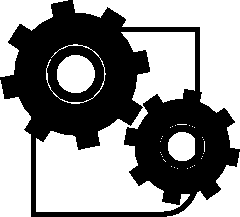
\includegraphics[width=0.75cm]{col11305.imgs/summary_simulation.png} &   \end{array} $ \hspace{2 pt}\raisebox{-5 pt}{} {(section shortcode: P10060 )} \par 
    \label{m38726*cid4}
            \subsection{ Balancing chemical equations}
            \nopagebreak
      \label{m38726*uid9}
            \subsubsection{ The law of conservation of mass}
            \nopagebreak
        \label{m38726*id63198}In order to balance a chemical equation, it is important to understand the law of conservation of mass.\par 
\label{m38726*fhsst!!!underscore!!!id145}\begin{definition}
	  \begin{tabular*}{15 cm}{m{15 mm}m{}}
	\hspace*{-50pt}  
\includegraphics[width=0.5in]{col11305.imgs/psflag2.png}   & \Definition{   \label{id2463440}\textbf{ The law of conservation of mass }} { \label{m38726*meaningfhsst!!!underscore!!!id145}
        \label{m38726*id63208}The mass of a closed system of substances will remain constant, regardless of the processes acting inside the system. Matter can change form, but cannot be created or destroyed. For any chemical process in a closed system, the mass of the reactants must equal the mass of the products. \par 
         } 
      \end{tabular*}
      \end{definition}
        \label{m38726*id63221}In a chemical equation then, the \textbf{mass} of the reactants must be equal to the mass of the products. In order to make sure that this is the case, the number of \textbf{atoms} of each element in the reactants must be equal to the number of atoms of those same elements in the products. Some examples are shown below:\par 
        \label{m38726*id63238}
          \textsl{Example 1:}
        \label{m38726*id63246}\nopagebreak\noindent{}
          
    \begin{equation}
    Fe+\mathrm{S}\to \mathrm{FeS}\tag{13.1}
      \end{equation}
        \par 
        \label{m38726*id63273}
    \setcounter{subfigure}{0}
	\begin{figure}[H] % horizontal\label{m38726*id63276}
    \begin{center}
    \label{m38726*id63276!!!underscore!!!media}\label{m38726*id63276!!!underscore!!!printimage}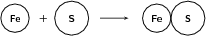
\includegraphics[width=5cm]{col11305.imgs/m38726_CG10C5_001.png} % m38726;CG10C5\_001.png;;;6.0;8.5;
      \vspace{2pt}
    \vspace{.1in}
    \end{center}
 \end{figure}       
        \par 
        \label{m38726*id63282}
          \textsl{Reactants}
        \par 
        \label{m38726*id63288}$\mathrm{Atomic\; mass\; of\; reactants}=55,8\phantom{\rule{2pt}{0ex}}u+32,1\phantom{\rule{2pt}{0ex}}u=\mathrm{87,9}\phantom{\rule{2pt}{0ex}}u$\par 
        \label{m38726*id63292}Number of atoms of each element in the reactants: $\left(1\ensuremath{\times}Fe\right)$ and $\left(1\ensuremath{\times}\mathrm{S}\right)$\par 
        \label{m38726*id63311}
          \textsl{Products}
        \par 
        \label{m38726*id63320}$\mathrm{Atomic\; mass\; of\; products}=55,8\phantom{\rule{2pt}{0ex}}u+32,1\phantom{\rule{2pt}{0ex}}u=\mathrm{87,9}\phantom{\rule{2pt}{0ex}}u$\par 
        \label{m38726*id63323}Number of atoms of each element in the products: $\left(1\ensuremath{\times}Fe\right)$ and $\left(1\ensuremath{\times}\mathrm{S}\right)$\par 
        \label{m38726*id63343}Since the number of atoms of each element is the same in the reactants and in the products, we say that the equation is \textbf{balanced}.\par 
        \label{m38726*id63352}
          \textsl{Example 2:}
        \label{m38726*id63361}\nopagebreak\noindent{}
          
    \begin{equation}
    {\mathrm{H}}_{2}+{\mathrm{O}}_{2}\to \mathrm{H}{}_{2}\mathrm{O}\tag{13.2}
      \end{equation}
        \par 
        \label{m38726*id63399}
    \setcounter{subfigure}{0}
	\begin{figure}[H] % horizontal\label{m38726*id63402}
    \begin{center}
    \label{m38726*id63402!!!underscore!!!media}\label{m38726*id63402!!!underscore!!!printimage}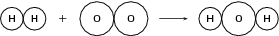
\includegraphics[width=5cm]{col11305.imgs/m38726_CG10C5_002.png} % m38726;CG10C5\_002.png;;;6.0;8.5;
      \vspace{2pt}
    \vspace{.1in}
    \end{center}
 \end{figure}       
        \par 
        \label{m38726*id63409}
          \textsl{Reactants}
        \par 
        \label{m38726*id63415}$\mathrm{Atomic\; mass\; of\; reactants}=\left(1+1\right)+\left(16+16\right)=\mathrm{34}\phantom{\rule{2pt}{0ex}}u$\par 
        \label{m38726*id63419}Number of atoms of each element in the reactants: $\left(2\ensuremath{\times}\mathrm{H}\right)$ and $\left(2\ensuremath{\times}\mathrm{O}\right)$\par 
        \label{m38726*id63438}
          \textsl{Product}
        \par 
        \label{m38726*id63446}$\mathrm{Atomic\; mass\; of\; product}=\left(1+1+16\right)=\mathrm{18}\phantom{\rule{2pt}{0ex}}u$\par 
        \label{m38726*id63450}Number of atoms of each element in the product: $\left(2\ensuremath{\times}\mathrm{H}\right)$ and $\left(1\ensuremath{\times}\mathrm{O}\right)$\par 
        \label{m38726*id63470}Since the total atomic mass of the reactants and the products is not the same and since there are more oxygen atoms in the reactants than there are in the product, the equation is \textbf{not balanced}.\par 
        \label{m38726*id63480}
          \textsl{Example 3:}
        \label{m38726*id63488}\nopagebreak\noindent{}
    \begin{equation}
    \mathrm{NaOH}+\mathrm{HCl}\to \mathrm{NaCl}+\mathrm{H}{}_{2}\mathrm{O}\tag{13.3}
      \end{equation}
        \par 
        \label{m38726*id63537}
    \setcounter{subfigure}{0}
	\begin{figure}[H] % horizontal\label{m38726*id63540}
    \begin{center}
    \label{m38726*id63540!!!underscore!!!media}\label{m38726*id63540!!!underscore!!!printimage}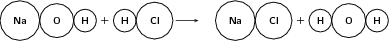
\includegraphics[width=300px]{col11305.imgs/m38726_CG10C5_003.png} % m38726;CG10C5\_003.png;;;6.0;8.5;
      \vspace{2pt}
    \vspace{.1in}
    \end{center}
 \end{figure}       
        \par 
        \label{m38726*id63546}
          \textsl{Reactants}
        \par 
        \label{m38726*id63553}$\mathrm{Atomic\; mass\; of\; reactants}=\left(23+6+1\right)+\left(1+35,4\right)=\mathrm{76,4}\phantom{\rule{2pt}{0ex}}u$\par 
        \label{m38726*id63556}Number of atoms of each element in the reactants: $\left(1\ensuremath{\times}\mathrm{Na}\right)+\left(1\ensuremath{\times}\mathrm{O}\right)+\left(2\ensuremath{\times}\mathrm{H}\right)+\left(1\ensuremath{\times}\mathrm{Cl}\right)$ \par 
        \label{m38726*id63592}
          \textsl{Products}
        \par 
        \label{m38726*id63600}$\mathrm{Atomic\; mass\; of\; products}=\left(23+35,4\right)+\left(1+1+16\right)=\mathrm{76,4}\phantom{\rule{2pt}{0ex}}u$\par 
        \label{m38726*id63604}Number of atoms of each element in the products: $\left(1\ensuremath{\times}\mathrm{Na}\right)+\left(1\ensuremath{\times}\mathrm{O}\right)+\left(2\ensuremath{\times}\mathrm{H}\right)+\left(1\ensuremath{\times}\mathrm{Cl}\right)$\par 
        \label{m38726*id63639}Since the number of atoms of each element is the same in the reactants and in the products, we say that the equation is \textbf{balanced}.\par 
        \label{m38726*id63649}We now need to find a way to balance those equations that are not balanced so that the number of atoms of each element in the reactants is the same as that for the products. This can be done by changing the \textbf{coefficients} of the molecules until the atoms on each side of the arrow are balanced. You will see later that these coefficients tell us something about the \textbf{mole ratio} in which substances react. They also tell us about the volume relationship between gases in the reactants and products.\par 
\label{m38726*notfhsst!!!underscore!!!id276}
\begin{tabular}{cc}
	   \hspace*{-50pt}\raisebox{-8 mm}{ 
\includegraphics[width=0.5in]{col11305.imgs/pstip2.png}  }& 
	\begin{minipage}{0.85\textwidth}
	\begin{note}
      {tip: }Coefficients
	\end{note}
	\end{minipage}
	\end{tabular}
	\par
        \label{m38726*id63674}Remember that if you put a number in front of a molecule, that number applies to the \textsl{whole} molecule. For example, if you write $2\mathrm{H}{}_{2}\mathrm{O}$, this means that there are 2 molecules of water. In other words, there are 4 hydrogen atoms and 2 oxygen atoms. If we write $3\mathrm{HCl}$, this means that there are 3 molecules of $\mathrm{HCl}$. In other words there are 3 hydrogen atoms and 3 chlorine atoms in total. In the first example, 2 is the coefficient and in the second example, 3 is the coefficient.\par 
      \label{m38726*eip-619}
            \subsubsection{ Activity: Balancing chemical equations}
            \nopagebreak
            \label{m38726*eip-695}You will need: coloured balls (or marbles), prestik, a sheet of paper and coloured pens.
\par 
\label{m38726*eip-69823}We will try to balance the following equation:
\label{m38726*eid0342}\nopagebreak\noindent{}
    \begin{equation}
    \mathrm{Al}+{\mathrm{O}}_{2}\to {\mathrm{Al}}_{2}{\mathrm{O}}_{3}\tag{13.4}
      \end{equation}
Take 1 ball of one colour. This represents a molecule of $Al$. Take two balls of another colour and stick them together. This represents a molecule of ${\mathrm{O}}_{2}$. Place these molecules on your left. Now take two balls of one colour and three balls of another colour to form a molecule of ${\mathrm{Al}}_{2}{\mathrm{O}}_{3}$. Place these molecules on your right. On a piece of paper draw coloured circles to represent the balls. Draw a line down the center of the paper to represent the molecules on the left and on the right. 
\par 
\label{m38726*id23534}
Count the number of balls on the left and the number on the right. Do you have the same number of each colour on both sides? If not the equation is not balanced. How many balls will you have to add to each side to make the number of balls the same? How would you add these balls?
\par 
\label{m38726*id09873432}You should find that you need 4 balls of one colour for $\mathrm{Al}$ and 3 pairs of balls of another colour (i.e. 6 balls in total) for ${\mathrm{O}}_{2}$ on the left side. On the right side you should find that you need 2 clusters of balls for ${\mathrm{Al}}_{2}{\mathrm{O}}_{3}$.
We say that the balanced equation is:
\label{m38726*id97235}\nopagebreak\noindent{}

    \begin{equation}
    4\mathrm{Al}+3{\mathrm{O}}_{2}\to 2{\mathrm{Al}}_{2}{\mathrm{O}}_{3}\tag{13.5}
      \end{equation}
\par 
\label{m38726*id570943}Repeat this process for the following reactions:
\label{m38726*id08342}\begin{itemize}[noitemsep]
            \item 
${\mathrm{CH}}_{4}+2{\mathrm{O}}_{2}\to {\mathrm{CO}}_{2}+2{\mathrm{H}}_{2}\mathrm{O}$
\item 
$2{\mathrm{H}}_{2}+{\mathrm{O}}_{2}\to 2{\mathrm{H}}_{2}\mathrm{O}$
\item 
$\mathrm{Zn}+2\mathrm{HCl}\to {\mathrm{ZnCl}}_{2}+{\mathrm{H}}_{2}$
\end{itemize}
\par \label{m38726*uid10}
            \subsubsection{ Steps to balance a chemical equation}
            \nopagebreak
        \label{m38726*id63708}When balancing a chemical equation, there are a number of steps that need to be followed.\par 
        \label{m38726*id63712}\begin{itemize}[noitemsep]
            \label{m38726*uid11}\item STEP 1: Identify the reactants and the products in the reaction and write their chemical formulae.
\label{m38726*uid12}\item STEP 2: Write the equation by putting the reactants on the left of the arrow and the products on the right.
\label{m38726*uid13}\item STEP 3: Count the number of atoms of each element in the reactants and the number of atoms of each element in the products.
\label{m38726*uid14}\item STEP 4: If the equation is not balanced, change the coefficients of the molecules until the number of atoms of each element on either side of the equation balance.
\label{m38726*uid15}\item STEP 5: Check that the atoms are in fact balanced.
\label{m38726*uid16}\item STEP 6 (we will look at this a little later): Add any extra details to the equation e.g. phase.
\end{itemize}
\par
            \label{m38726*secfhsst!!!underscore!!!id296}\vspace{.5cm} 
      \noindent
      \hspace*{-30pt}
\includegraphics[width=0.5in]{col11305.imgs/pspencil2.png}   \raisebox{25mm}{   
      \begin{mdframed}[linewidth=4, leftmargin=40, rightmargin=40]  
      \begin{exercise}
    \noindent\textbf{Exercise 13.1:  Balancing chemical equations 1 }
        \label{m38726*probfhsst!!!underscore!!!id297}
        \label{m38726*id63803}Balance the following equation:
        \label{m38726*id63808}\nopagebreak\noindent{}
    \begin{equation}
    \mathrm{Mg}+\mathrm{HCl}\to {\mathrm{MgCl}}_{2}+{\mathrm{H}}_{2}\tag{13.6}
      \end{equation}
        \par 
        \vspace{5pt}
        \label{m38726*solfhsst!!!underscore!!!id327}\noindent\textbf{Solution to Exercise } \label{m38726*listfhsst!!!underscore!!!id327}\begin{enumerate}[noitemsep, label=\textbf{Step} \textbf{\arabic*}. ] 
            \leftskip=20pt\rightskip=\leftskip\item  
        \label{m38726*id63895}Reactants: $\mathrm{Mg}=1\phantom{\rule{2pt}{0ex}}\mathrm{atom}$; $\mathrm{H}=1\phantom{\rule{2pt}{0ex}}\mathrm{atom}$ and $\mathrm{Cl}=1\phantom{\rule{2pt}{0ex}}\mathrm{atom}$\par 
        \label{m38726*id63899}Products: $\mathrm{Mg}=1\phantom{\rule{2pt}{0ex}}\mathrm{atom}$; $\mathrm{H}=2\phantom{\rule{2pt}{0ex}}\mathrm{atoms}$ and $\mathrm{Cl}=2\phantom{\rule{2pt}{0ex}}\mathrm{atoms}$\par 
        \item  
        \label{m38726*id63906}The equation is not balanced since there are 2 chlorine atoms in the product and only 1 in the reactants. If we add a coefficient of 2 to the $\mathrm{HCl}$ to increase the number of $\mathrm{H}$ and $\mathrm{Cl}$ atoms in the reactants, the equation will look like this:
        \label{m38726*id63912}\nopagebreak\noindent{} 
    \begin{equation}
    \mathrm{Mg}+2\mathrm{HCl}\to {\mathrm{MgCl}}_{2}+{\mathrm{H}}_{2}\tag{13.7}
      \end{equation}
        \par 
        \item  
        \label{m38726*id63970}If we count the atoms on each side of the equation, we find the following:\par 
        \label{m38726*id63974}Reactants: $\mathrm{Mg}=1\phantom{\rule{2pt}{0ex}}\mathrm{atom}$; $\mathrm{H}=2\phantom{\rule{2pt}{0ex}}\mathrm{atom}$ and $\mathrm{Cl}=2\phantom{\rule{2pt}{0ex}}\mathrm{atom}$\par 
        \label{m38726*id63977}Products: $\mathrm{Mg}=1\phantom{\rule{2pt}{0ex}}\mathrm{atom}$; $\mathrm{H}=2\phantom{\rule{2pt}{0ex}}\mathrm{atom}$ and $\mathrm{Cl}=2\phantom{\rule{2pt}{0ex}}\mathrm{atom}$\par 
        \label{m38726*id63981}The equation is balanced. The final equation is:
        \label{m38726*id643712}\nopagebreak\noindent{} 
    \begin{equation}
    \mathrm{Mg}+2\mathrm{HCl}\to {\mathrm{MgCl}}_{2}+{\mathrm{H}}_{2}\tag{13.8}
      \end{equation}
        \par 
 \end{enumerate}
    \end{exercise}
    \end{mdframed}
    }
    \noindent
\par
            \label{m38726*secfhsst!!!underscore!!!id394}\vspace{.5cm} 
      \noindent
      \hspace*{-30pt}
\includegraphics[width=0.5in]{col11305.imgs/pspencil2.png}   \raisebox{25mm}{   
      \begin{mdframed}[linewidth=4, leftmargin=40, rightmargin=40]  
      \begin{exercise}
    \noindent\textbf{Exercise 13.2:  Balancing chemical equations 2 }
        \label{m38726*probfhsst!!!underscore!!!id395}
        \label{m38726*id64047}Balance the following equation:
        \label{m38726*id64052}\nopagebreak\noindent{}
        
    \begin{equation}
    {\mathrm{CH}}_{4}+{\mathrm{O}}_{2}\to {\mathrm{CO}}_{2}+\mathrm{H}{}_{2}\mathrm{O}\tag{13.9}
      \end{equation}
        \par 
        \vspace{5pt}
        \label{m38726*solfhsst!!!underscore!!!id427}\noindent\textbf{Solution to Exercise } \label{m38726*listfhsst!!!underscore!!!id427}\begin{enumerate}[noitemsep, label=\textbf{Step} \textbf{\arabic*}. ] 
            \leftskip=20pt\rightskip=\leftskip\item  
        \label{m38726*id64139}Reactants: $\mathrm{C}=1$; $\mathrm{H}=4$ and $\mathrm{O}=2$\par 
        \label{m38726*id64142}Products: $\mathrm{C}=1$; $\mathrm{H}=2$ and $\mathrm{O}=3$\par 
        \item  
        \label{m38726*id64149}If we add a coefficient of 2 to $\mathrm{H}{}_{2}\mathrm{O}$, then the number of hydrogen atoms in the reactants will be 4, which is the same as for the reactants. The equation will be:
       \label{m38726*id6852}\nopagebreak\noindent{}
        
    \begin{equation}
    {\mathrm{CH}}_{4}+{\mathrm{O}}_{2}\to {\mathrm{CO}}_{2}+2\mathrm{H}{}_{2}\mathrm{O}\tag{13.10}
      \end{equation}
        \par 
        \item  
        \label{m38726*id64230}Reactants: $\mathrm{C}=1$; $\mathrm{H}=4$ and $\mathrm{O}=2$\par 
        \label{m38726*id64234}Products: $\mathrm{C}=1$; $\mathrm{H}=4$ and $\mathrm{O}=4$ \par 
        \label{m38726*id64238}You will see that, although the number of \textsl{hydrogen} atoms now balances, there are more oxygen atoms in the products. You now need to repeat the previous step. If we put a coefficient of 2 in front of $\mathrm{O}{}_{2}$, then we will increase the number of oxygen atoms in the reactants by 2. The new equation is:
        \label{m38726*id644352}\nopagebreak\noindent{}
        
    \begin{equation}
    {\mathrm{CH}}_{4}+2{\mathrm{O}}_{2}\to {\mathrm{CO}}_{2}+2\mathrm{H}{}_{2}\mathrm{O}\tag{13.11}
      \end{equation}
        \par 
        \label{m38726*id64320}When we check the number of atoms again, we find that the number of atoms of each element in the reactants is the same as the number in the products. The equation is now balanced.\par 
 \end{enumerate}
    \end{exercise}
    \end{mdframed}
    }
    \noindent
\label{m38726*secfhsst!!!underscore!!!id501}\vspace{.5cm} 
      \noindent
      \hspace*{-30pt}
\includegraphics[width=0.5in]{col11305.imgs/pspencil2.png}   \raisebox{25mm}{   
      \begin{mdframed}[linewidth=4, leftmargin=40, rightmargin=40]  
      \begin{exercise}
    \noindent\textbf{Exercise 13.3:  Balancing chemical equations 3 }
        \label{m38726*probfhsst!!!underscore!!!id502}
        \label{m38726*id64337}Nitrogen gas reacts with hydrogen gas to form ammonia. Write a balanced chemical equation for this reaction.\par 
        \vspace{5pt}
        \label{m38726*solfhsst!!!underscore!!!id506}\noindent\textbf{Solution to Exercise } \label{m38726*listfhsst!!!underscore!!!id506}\begin{enumerate}[noitemsep, label=\textbf{Step} \textbf{\arabic*}. ] 
            \leftskip=20pt\rightskip=\leftskip\item  
        \label{m38726*id64383}The reactants are nitrogen ($\mathrm{N}{}_{2}$) and hydrogen ($\mathrm{H}{}_{2}$) and the product is ammonia ($\mathrm{NH}{}_{3}$).\par 
        \item  
        \label{m38726*id64433}The equation is as follows:
        \label{m38726*id76543}\nopagebreak\noindent{}
        
    \begin{equation}
    {\mathrm{N}}_{2}+{\mathrm{H}}_{2}\to {\mathrm{NH}}_{3}\tag{13.12}
      \end{equation}
        \par 
        \item  
        \label{m38726*id64485}Reactants: $\mathrm{N}=2$ and $\mathrm{H}=2$\par 
        \label{m38726*id64488}Products: $\mathrm{N}=1$ and $\mathrm{H}=3$\par 
        \item  
        \label{m38726*id64495}In order to balance the number of nitrogen atoms, we could rewrite the equation as:
        \label{m38726*id798543}\nopagebreak\noindent{}
        
    \begin{equation}
    {\mathrm{N}}_{2}+{\mathrm{H}}_{2}\to 2{\mathrm{NH}}_{3}\tag{13.13}
      \end{equation}
        \par 
        \item  
        \label{m38726*id64550}In the above equation, the nitrogen atoms now balance, but the hydrogen atoms don't (there are 2 hydrogen atoms in the reactants and 6 in the product). If we put a coefficient of 3 in front of the hydrogen (${\mathrm{H}}_{2}$), then the hydrogen atoms and the nitrogen atoms balance. The final equation is:
              \label{m38726*id756543}\nopagebreak\noindent{}
        
    \begin{equation}
    {\mathrm{N}}_{2}+3{\mathrm{H}}_{2}\to 2{\mathrm{NH}}_{3}\tag{13.14}
      \end{equation}
        \par 
\end{enumerate}
    \end{exercise}
    \end{mdframed}
    }
    \noindent
\par
            \label{m38726*secfhsst!!!underscore!!!id590}\vspace{.5cm} 
      \noindent
      \hspace*{-30pt}
\includegraphics[width=0.5in]{col11305.imgs/pspencil2.png}   \raisebox{25mm}{   
      \begin{mdframed}[linewidth=4, leftmargin=40, rightmargin=40]  
      \begin{exercise}
    \noindent\textbf{Exercise 13.4:  Balancing chemical equations 4 }
        \label{m38726*probfhsst!!!underscore!!!id591}
        \label{m38726*id64630}In our bodies, sugar (${\mathrm{C}}_{6}{\mathrm{H}}_{12}{\mathrm{O}}_{6}$) reacts with the oxygen we breathe in to produce carbon dioxide, water and energy. Write the balanced equation for this reaction.\par 
        \vspace{5pt}
        \label{m38726*solfhsst!!!underscore!!!id595}\noindent\textbf{Solution to Exercise } \label{m38726*listfhsst!!!underscore!!!id595}\begin{enumerate}[noitemsep, label=\textbf{Step} \textbf{\arabic*}. ] 
            \leftskip=20pt\rightskip=\leftskip\item  
        \label{m38726*id64715}Reactants: sugar (${\mathrm{C}}_{6}{\mathrm{H}}_{12}{\mathrm{O}}_{6}$) and oxygen (${\mathrm{O}}_{2}$)\par 
        \label{m38726*id64778}Products: carbon dioxide (${\mathrm{CO}}_{2}$) and water ($\mathrm{H}{}_{2}\mathrm{O}$)\par 
        \item  
        \label{m38726*uid097212}\nopagebreak\noindent{}
    \begin{equation}
    {\mathrm{C}}_{6}{\mathrm{H}}_{12}{\mathrm{O}}_{6}+{\mathrm{O}}_{2}\to {\mathrm{CO}}_{2}+\mathrm{H}{}_{2}\mathrm{O}\tag{13.15}
      \end{equation}
        \item  
        \label{m38726*id64900}Reactants: $\mathrm{C}=6$; $\mathrm{H}=12$ and $\mathrm{O}=8$ \par 
        \label{m38726*id64903}Products: $\mathrm{C}=1$; $\mathrm{H}=2$ and $\mathrm{O}=3$\par 
        \item  
        \label{m38726*id64912}It is easier to start with carbon as it only appears once on each side. If we add a 6 in front of ${\mathrm{CO}}_{2}$, the equation looks like this:
\label{m38726*uid0913}\nopagebreak\noindent{}

    \begin{equation}
    {\mathrm{C}}_{6}{\mathrm{H}}_{12}{\mathrm{O}}_{6}+{\mathrm{O}}_{2}\to 6{\mathrm{CO}}_{2}+\mathrm{H}{}_{2}\mathrm{O}\tag{13.16}
      \end{equation}
    \par 
        \label{m38726*id64998}Reactants: $\mathrm{C}=6$; $\mathrm{H}=12$ and $\mathrm{O}=8$\par 
        \label{m38726*id65004}Products: $\mathrm{C}=6$; $\mathrm{H}=2$ and $\mathrm{O}=13$\par 
        \item  
        \label{m38726*id65011}Let's try to get the number of hydrogens the same this time.
\label{m38726*uid0987213}\nopagebreak\noindent{}

    \begin{equation}
    {\mathrm{C}}_{6}{\mathrm{H}}_{12}{\mathrm{O}}_{6}+{\mathrm{O}}_{2}\to 6{\mathrm{CO}}_{2}+6\mathrm{H}{}_{2}\mathrm{O}\tag{13.17}
      \end{equation}
\par 
        \label{m38726*id65085}Reactants: $\mathrm{C}=6$; $\mathrm{H}=12$ and $\mathrm{O}=8$\par 
        \label{m38726*id65091}Products: $\mathrm{C}=6$; $\mathrm{H}=12$ and $\mathrm{O}=18$ \par 
        \item  
\label{m38726*uid091873}\nopagebreak\noindent{}

    \begin{equation}
    {\mathrm{C}}_{6}{\mathrm{H}}_{12}{\mathrm{O}}_{6}+12{\mathrm{O}}_{2}\to 6{\mathrm{CO}}_{2}+6\mathrm{H}{}_{2}\mathrm{O}\tag{13.18}
      \end{equation}
        \label{m38726*id65171}Reactants: $\mathrm{C}=6$; $\mathrm{H}=12$ and $\mathrm{O}=18$\par 
        \label{m38726*id65176}Products: $\mathrm{C}=6$; $\mathrm{H}=12$ and $\mathrm{O}=18$\par 
 \end{enumerate}
    \end{exercise}
    \end{mdframed}
    }
    \noindent
This simulation allows you to practice balancing simple equations.
   \setcounter{subfigure}{0}
	\begin{figure}[H] % horizontal\label{m38806*transverse-waves}
    \textnormal{Phet simulation for balancing equations}\vspace{.1in} \nopagebreak
  \label{m38806*phet!!!underscore!!!sim}\label{m38806*phet-simulation}
            \raisebox{-5 pt}{ 
\includegraphics[width=0.5cm]{col11305.imgs/summary_www.png}} { (Simulation:  lbD )}
      \vspace{2pt}
    \vspace{.1in}
 \end{figure}       
        \par \label{m38726*secfhsst!!!underscore!!!id763}
            \subsubsection{  Balancing simple chemical equations
        }
            \nopagebreak
        \label{m38726*id65193}Balance the following equations:\par 
        \label{m38726*id65199}\begin{enumerate}[noitemsep, label=\textbf{\arabic*}. ] 
            \label{m38726*uid17}\item Hydrogen fuel cells are extremely important in the development of alternative energy sources. Many of these cells work by reacting hydrogen and oxygen gases together to form water, a reaction which also produces electricity. Balance the following equation: ${{H}}_{2}\left(\mathrm{g}\right)+{{O}}_{2}\left(\mathrm{g}\right)\to \mathrm{H}{}_{2}\mathrm{O}\left(\mathrm{l}\right)$        \label{m38726*uid18}\item The synthesis of ammonia ($\mathrm{NH}{}_{3}$), made famous by the German chemist Fritz Haber in the early 20th century, is one of the most important reactions in the chemical industry. Balance the following equation used to produce ammonia:
${{N}}_{2}\left(\mathrm{g}\right)+{{H}}_{2}\left(\mathrm{g}\right)\to \mathrm{NH}{}_{3}\left(\mathrm{g}\right)$
        \label{m38726*uid19}\item 
          ${Mg}+{{P}}_{4}\to \mathrm{Mg}{}_{3}{\mathrm{P}}_{2}$
        \label{m38726*uid20}\item 
          ${Ca}+{{H}}_{2}\mathrm{O}\to \mathrm{Ca\left(OH\right)}{}_{2}+\mathrm{H}{}_{2}$        \label{m38726*uid21}\item 
          ${{CuCO}}_{3}+{{H}}_{2}{\mathrm{SO}}_{4}\to \mathrm{CuSO}{}_{4}+{{H}}_{2}\mathrm{O}+{{CO}}_{2}$
        \label{m38726*uid22}\item 
          ${{CaCl}}_{2}+{{Na}}_{2}{\mathrm{CO}}_{3}\to \mathrm{CaCO}{}_{3}+{NaCl}$        \label{m38726*uid23}\item 
          ${\mathrm{C}}_{12}{\mathrm{H}}_{22}{\mathrm{O}}_{11}+{{O}}_{2}\to \mathrm{H}{}_{2}\mathrm{O}+{{CO}}_{2}$
          \hspace{1ex}        \label{m38726*uid24}\item Barium chloride reacts with sulphuric acid to produce barium sulphate and hydrochloric acid.
        \label{m38726*uid25}\item Ethane (${\mathrm{C}}_{2}{\mathrm{H}}_{6}$) reacts with oxygen to form carbon dioxide and steam.
        \label{m38726*uid26}\item Ammonium carbonate is often used as a smelling salt. Balance the following reaction for the decomposition of ammonium carbonate:
$\left({\mathrm{NH}}_{4}\right){}_{2}{\mathrm{CO}}_{3}\left(\mathrm{s}\right)\to {\mathrm{NH}}_{3}\left(\mathrm{aq}\right)+{\mathrm{CO}}_{2}\left(\mathrm{g}\right)+\mathrm{H}{}_{2}\mathrm{O}\left(\mathrm{l}\right)$\hspace{1ex}        \end{enumerate}
  \label{m38726**end}
\par \raisebox{-5 pt}{
\includegraphics[width=0.5cm]{col11305.imgs/summary_www.png}} Find the answers with the shortcodes:
 \par \begin{tabular}[h]{cccccc}
 (1.) lOg  &  (2.) lO4  &  (3.) lO2  &  (4.) lOT  &  (5.) lOb  &  (6.) lOj  &  (7.) lOD  &  (8.) lOW  &  (9.) lOZ  &  (10.) lOB  & \end{tabular}
         \section{ State symbols}
    \nopagebreak
            \label{m38727} $ \hspace{-5pt}\begin{array}{cccccccccccc}   
\includegraphics[width=0.75cm]{col11305.imgs/summary_fullmarks.png} &   
\includegraphics[width=0.75cm]{col11305.imgs/summary_video.png} &   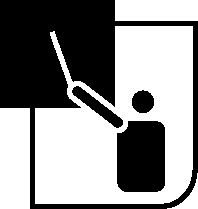
\includegraphics[width=0.75cm]{col11305.imgs/summary_presentation.png} &   \end{array} $ \hspace{2 pt}\raisebox{-5 pt}{} {(section shortcode: P10061 )} \par 
    \label{m38727*cid5}
            \subsection{ State symbols and other information}
            \nopagebreak
      \label{m38727*id65920}The state (phase) of the compounds can be expressed in the chemical equation. This is done by placing the correct label on the right hand side of the formula. There are only four labels that can be used:\par 
      \label{m38727*id65925}\begin{enumerate}[noitemsep, label=\textbf{\arabic*}. ] 
            \label{m38727*uid27}\item (g) for gaseous compounds
\label{m38727*uid28}\item (l) for liquids
\label{m38727*uid29}\item (s) for solid compounds
\label{m38727*uid30}\item (aq) for an aqueous (water) solution
\end{enumerate}
\label{m38727*eip-536}To show that heat is needed for a reaction, a Greek delta ($\Delta $) is placed above the arrow.\par \label{m38727*notfhsst!!!underscore!!!id966}
\begin{tabular}{cc}
	   \hspace*{-50pt}\raisebox{-8 mm}{ 
\includegraphics[width=0.5in]{col11305.imgs/pstip2.png}  }& 
	\begin{minipage}{0.85\textwidth}
	\begin{note}
      {tip: }You may remember from Physical and chemical change\footnote{\raggedright{}"Physical and Chemical Change - Grade 10 [CAPS]" <http://http://cnx.org/content/m38141/latest/>} that energy cannot be created or destroyed during a chemical reaction but it may change form. In an exothermic reaction, $\Delta $H is less than zero and in an endothermic reaction, $\Delta $H is greater than zero. This value is often written at the end of a chemical equation.
	\end{note}
	\end{minipage}
	\end{tabular}
	\par
\label{m38727*secfhsst!!!underscore!!!id967}\vspace{.5cm} 
      \noindent
      \hspace*{-30pt}
\includegraphics[width=0.5in]{col11305.imgs/pspencil2.png}   \raisebox{25mm}{   
      \begin{mdframed}[linewidth=4, leftmargin=40, rightmargin=40]  
      \begin{exercise}
    \noindent\textbf{Exercise 13.5: Balancing chemical equations 5}\label{m38727*probfhsst!!!underscore!!!id968}
      \label{m38727*id66044}Solid zinc metal reacts with aqueous hydrochloric acid to form an aqueous solution of zinc chloride ($\mathrm{ZnCl}{}_{2}$)and hydrogen gas. Write a balanced equation for this reaction.\par 
      \vspace{5pt}
      \label{m38727*solfhsst!!!underscore!!!id972}\noindent\textbf{Solution to Exercise } \label{m38727*listfhsst!!!underscore!!!id972}\begin{enumerate}[noitemsep, label=\textbf{Step} \textbf{\arabic*}. ] 
            \leftskip=20pt\rightskip=\leftskip\item  
      \label{m38727*id66103}The reactants are zinc ($\mathrm{Zn}$) and hydrochloric acid ($\mathrm{HCl}$). The products are zinc chloride ($\mathrm{ZnCl}{}_{2}$) and hydrogen ($\mathrm{H}{}_{2}$).\par 
      \item  
      \label{m38727*id66139}\nopagebreak\noindent{}
      
    \begin{equation}
    \mathrm{Zn}+\mathrm{HCl}\to \mathrm{ZnCl}{}_{2}+\mathrm{H}{}_{2}\tag{13.19}
      \end{equation}
      \item  
      \label{m38727*id66196}You will notice that the zinc atoms balance but the chlorine and hydrogen atoms don't. Since there are two chlorine atoms on the right and only one on the left, we will give $\mathrm{HCl}$ a coefficient of 2 so that there will be two chlorine atoms on each side of the equation.
      \label{m38727*id66202}\nopagebreak\noindent{}
      
    \begin{equation}
    \mathrm{Zn}+2\mathrm{HCl}\to \mathrm{ZnCl}{}_{2}+\mathrm{H}{}_{2}\tag{13.20}
      \end{equation}
      \par 
      \item  
      \label{m38727*id66262}When you look at the equation again, you will see that all the atoms are now balanced.\par 
      \item  
      \label{m38727*id66270}In the initial description, you were told that zinc was a metal, hydrochloric acid and zinc chloride were in aqueous solutions and hydrogen was a gas.
      \label{m38727*id66274}\nopagebreak\noindent{}
      
    \begin{equation}
    \mathrm{Zn}\left(\mathrm{s}\right)+2\mathrm{HCl}\left(\mathrm{aq}\right)\to \mathrm{ZnCl}{}_{2}\left(\mathrm{aq}\right)+\mathrm{H}{}_{2}\left(\mathrm{g}\right)\tag{13.21}
      \end{equation}
      \par 
\end{enumerate}
    \end{exercise}
    \end{mdframed}
    }
    \noindent
\par \pagebreak
            \label{m38727*secfhsst!!!underscore!!!id1086}\vspace{.5cm} 
      \noindent
      \hspace*{-30pt}
\includegraphics[width=0.5in]{col11305.imgs/pspencil2.png}   \raisebox{25mm}{   
      \begin{mdframed}[linewidth=4, leftmargin=40, rightmargin=40]  
      \begin{exercise}
    \noindent\textbf{Exercise 13.6:  Balancing chemical equations 5 (advanced) }
      \label{m38727*probfhsst!!!underscore!!!id1087}
      \label{m38727*id66373}Balance the following equation:
      \label{m38727*id66378}\nopagebreak\noindent{}
      
    \begin{equation}
    \left({\mathrm{NH}}_{4}\right){}_{2}{\mathrm{SO}}_{4}+\mathrm{NaOH}\to \mathrm{NH}{}_{3}+\mathrm{H}{}_{2}\mathrm{O}+\mathrm{Na}{}_{2}{\mathrm{SO}}_{4}\tag{13.22}
      \end{equation}
      \par 
      \label{m38727*id66476}In this example, the first two steps are not necessary because the reactants and products have already been given.\par 
      \vspace{5pt}
      \label{m38727*solfhsst!!!underscore!!!id1143}\noindent\textbf{Solution to Exercise } \label{m38727*listfhsst!!!underscore!!!id1143}\begin{enumerate}[noitemsep, label=\textbf{Step} \textbf{\arabic*}. ] 
            \leftskip=20pt\rightskip=\leftskip\item  
      \label{m38727*id66518}With a complex equation, it is always best to start with atoms that appear only once on each side i.e. $\mathrm{Na}$, $\mathrm{N}$ and $\mathrm{S}$ atoms. Since the $\mathrm{S}$ atoms already balance, we will start with $\mathrm{Na}$ and $\mathrm{N}$ atoms. There are two $\mathrm{Na}$ atoms on the right and one on the left. We will add a second $\mathrm{Na}$ atom by giving $\mathrm{NaOH}$ a coefficient of two. There are two $\mathrm{N}$ atoms on the left and one on the right. To balance the $\mathrm{N}$ atoms, $\mathrm{NH}{}_{3}$ will be given a coefficient of two. The equation now looks as follows:
      \label{m38727*id66539}\nopagebreak\noindent{}
      
    \begin{equation}
    \left({\mathrm{NH}}_{4}\right){}_{2}{\mathrm{SO}}_{4}+2\mathrm{NaOH}\to 2\mathrm{NH}{}_{3}+\mathrm{H}{}_{2}\mathrm{O}+\mathrm{Na}{}_{2}{\mathrm{SO}}_{4}\tag{13.23}
      \end{equation}
      \par 
      \item  
      \label{m38727*id66648}$\mathrm{N}$, $\mathrm{Na}$ and $\mathrm{S}$ atoms balance, but $\mathrm{O}$ and $\mathrm{H}$ atoms do not. There are six $\mathrm{O}$ atoms and ten $\mathrm{H}$ atoms on the left, and five $\mathrm{O}$ atoms and eight $\mathrm{H}$ atoms on the right. We need to add one $\mathrm{O}$ atom and two $\mathrm{H}$ atoms on the right to balance the equation. This is done by adding another $\mathrm{H}{}_{2}\mathrm{O}$ molecule on the right hand side. We now need to check the equation again:
      \label{m38727*id66667}\nopagebreak\noindent{}
      
    \begin{equation}
    \left({\mathrm{NH}}_{4}\right){}_{2}{\mathrm{SO}}_{4}+2\mathrm{NaOH}\to 2\mathrm{NH}{}_{3}+2\mathrm{H}{}_{2}\mathrm{O}+\mathrm{Na}{}_{2}{\mathrm{SO}}_{4}\tag{13.24}
      \end{equation}
      \par 
      \label{m38727*id66774}The equation is now balanced.\par 
\end{enumerate}
    \end{exercise}
    \end{mdframed}
    }
    \noindent
\label{m38727*eip-44}The following video explains some of the concepts of balancing chemical equations.\newline
    \setcounter{subfigure}{0}
	\begin{figure}[H] % horizontal\label{m38727*balancing-equations}
    \textnormal{Khan Academy video on balancing chemical equations}\vspace{.1in} \nopagebreak
  \label{m38727*yt-media1}\label{m38727*yt-video1}
            \raisebox{-5 pt}{ 
\includegraphics[width=0.5cm]{col11305.imgs/summary_www.png}} { (Video:  P10062 )}
      \vspace{2pt}
    \vspace{.1in}
 \end{figure}       \par \label{m38727*secfhsst!!!underscore!!!id1261}
            \subsubsection{  Balancing more advanced chemical equations
      }
            \nopagebreak
      \label{m38727*id66790}Write balanced equations for each of the following reactions:\par 
      \label{m38727*id66796}\begin{enumerate}[noitemsep, label=\textbf{\arabic*}. ] 
            \label{m38727*uid31}\item 
${Al}_{2}{\mathrm{O}}_{3}\left(\mathrm{s}\right)+{\mathrm{H}}_{2}{\mathrm{SO}}_{4}\left(\mathrm{aq}\right)\to {Al}_{2}\left({\mathrm{SO}}_{4}\right){}_{3}\left(\mathrm{aq}\right)+3{{H}}_{2}{O}\left(\mathrm{l}\right)$
        \label{m38727*uid32}\item 
        ${\mathrm{Mg\left(OH\right)}}_{2}\left(\mathrm{aq}\right)+{\mathrm{HNO}}_{3}\left(\mathrm{aq}\right)\to Mg\left({\mathrm{NO}}_{3}\right){}_{2}\left(\mathrm{aq}\right)+2{{H}}_{2}{O}\left(\mathrm{l}\right)$
        \label{m38727*uid33}\item Lead (II) nitrate solution reacts with potassium iodide solution.
\label{m38727*uid34}\item When heated, aluminium reacts with solid copper oxide to produce copper metal and aluminium oxide (${Al}_{2}{\mathrm{O}}_{3}$).
\label{m38727*uid35}\item When calcium chloride solution is mixed with silver nitrate solution, a white precipitate (solid) of silver chloride appears. Calcium nitrate ($Ca\left({\mathrm{NO}}_{3}\right){}_{2}$) is also produced in the solution.
        \end{enumerate}
    \label{m38727*eip-429}Balanced equations are very important in chemistry. It is only by working with the balanced equations that chemists can perform many different calculations that tell them what quantity of something reacts. In a later chapter we will learn how to work with some of these calculations. We can interpret balanced chemical equations in terms of the conservation of matter, the conservation of mass or the conservation of energy. \label{m38727*eip-366}
    \setcounter{subfigure}{0}
	\begin{figure}[H] % horizontal\label{m38727*slidesharefigure}
    \label{m38727*slidesharemedia}\label{m38727*slideshareflash}\raisebox{-5 pt}{ 
\includegraphics[width=0.5cm]{col11305.imgs/summary_www.png}} { (Presentation:  P10063 )}
      \vspace{2pt}
    \vspace{.1in}
 \end{figure}       \par \label{m38727*cid6}
\par \raisebox{-5 pt}{
\includegraphics[width=0.5cm]{col11305.imgs/summary_www.png}} Find the answers with the shortcodes:
 \par \begin{tabular}[h]{cccccc}
 (1.) lOK  & \end{tabular}
            \subsection{ Summary}
            \nopagebreak
      \label{m38727*id67171}\begin{itemize}[noitemsep]
            \label{m38727*uid36}\item A \textbf{chemical equation} uses symbols to describe a chemical reaction.
\label{m38727*uid37}\item In a chemical equation, \textbf{reactants} are written on the left hand side of the equation and the \textbf{products} on the right. The arrow is used to show the direction of the reaction.
\label{m38727*uid38}\item When representing chemical change, it is important to be able to write the \textbf{chemical formula} of a compound.
\label{m38727*uid39}\item In any chemical reaction, the \textbf{law of conservation of mass} applies. This means that the total atomic mass of the reactants must be the same as the total atomic mass of the products. This also means that the number of atoms of each element in the reactants must be the same as the number of atoms of each element in the product.
\label{m38727*uid40}\item If the number of atoms of each element in the reactants is the same as the number of atoms of each element in the product, then the equation is \textbf{balanced}.
\label{m38727*uid41}\item If the number of atoms of each element in the reactants is not the same as the number of atoms of each element in the product, then the equation is \textbf{not balanced}.
\label{m38727*uid42}\item In order to balance an equation, \textbf{coefficients} can be placed in front of the reactants and products until the number of atoms of each element is the same on both sides of the equation.
\end{itemize}
\label{m38727*secfhsst!!!underscore!!!id1434}
            \subsubsection{ End of chapter exercises      }
            \nopagebreak
      \label{m38727*id67334}\begin{enumerate}[noitemsep, label=\textbf{\arabic*}. ] 
            \label{m38727*uid45}\item Propane is a fuel that is commonly used as a heat source for engines and homes. Balance the following equation for the combustion of propane:
        ${\mathrm{C}}_{3}{\mathrm{H}}_{8}\left(\mathrm{l}\right)+\mathrm{O}{}_{2}\left(\mathrm{g}\right)\to \mathrm{CO}{}_{2}\left(\mathrm{g}\right)+\mathrm{H}{}_{2}\mathrm{O}\left(\mathrm{l}\right)$
        \label{m38727*uid46}\item Aspartame, an artificial sweetener, has the formula ${\mathrm{C}}_{14}{\mathrm{H}}_{18}{\mathrm{N}}_{2}{\mathrm{O}}_{2}$. Write the balanced equation for its combustion (reaction with ${\mathrm{O}}_{2}$) to form ${\mathrm{CO}}_{2}$ gas, liquid $\mathrm{H}{}_{2}\mathrm{O}$, and ${\mathrm{N}}_{2}$ gas.
        \label{m38727*uid47}\item 
${Fe}_{2}\left({\mathrm{SO}}_{4}\right){}_{3}+\mathrm{K\left(SCN\right)}\to {\mathrm{K}}_{3}{\mathrm{Fe\left(SCN\right)}}_{6}+{\mathrm{K}}_{2}{\mathrm{SO}}_{4}$
                \label{m38727*uid48}\item Chemical weapons were banned by the Geneva Protocol in 1925. According to this protocol, all chemicals that release suffocating and poisonous gases are not to be used as weapons. White phosphorus, a very reactive allotrope of phosphorus, was recently used during a military attack. Phosphorus burns vigorously in oxygen. Many people got severe burns and some died as a result. The equation for this spontaneous reaction is:
        ${\mathrm{P}}_{4}\left(\mathrm{s}\right)+{\mathrm{O}}_{2}\left(\mathrm{g}\right)\to {\mathrm{P}}_{2}{\mathrm{O}}_{5}\left(\mathrm{s}\right)$\label{m38727*id67821}\begin{enumerate}[noitemsep, label=\textbf{\alph*}. ] 
            \label{m38727*uid49}\item Balance the chemical equation.
\label{m38727*uid50}\item Prove that the law of conservation of mass is obeyed during this chemical reaction.
\label{m38727*uid51}\item Name the product formed during this reaction.
\label{m38727*uid52}\item Classify the reaction as endothermic or exothermic. Give a reason for your answer.
\label{m38727*uid53}\item Classify the reaction as a synthesis or decomposition reaction. Give a reason for your answer.
        \end{enumerate}
(DoE Exemplar Paper 2 2007)
\item Mixing bleach ($\mathrm{NaOCl}$) and ammonia (two common household cleaners) is very dangerous. When these two substances are mixed they produce toxic chloaramine (${\mathrm{NH}}_{2}Cl$) fumes. Balance the following equations that occur when bleach and ammonia are mixed:\label{m38727*id6432}\begin{enumerate}[noitemsep, label=\textbf{\alph*}. ] 
            \item $\mathrm{NaOCl}\left(\mathrm{aq}\right)+{\mathrm{NH}}_{3}\left(\mathrm{aq}\right)\to {\mathrm{NaONH}}_{3}\left(\mathrm{aq}\right)+{Cl}_{2}\left(\mathrm{g}\right)$\item If there is more bleach than ammonia the following may occur:
$\mathrm{NaOCl}+{\mathrm{NH}}_{3}\to \mathrm{NaOH}+{\mathrm{NCl}}_{3}$
\newline
    Nitrogen trichloride (${\mathrm{NCl}}_{3}$) is highly explosive.\item If there is more ammonia than bleach the following may occur:
${\mathrm{NH}}_{3}+\mathrm{NaOCl}\to \mathrm{NaOH}+{\mathrm{NH}}_{2}Cl$\newline
These two products then react with ammonia as follows:\newline
${\mathrm{NH}}_{3}+{\mathrm{NH}}_{2}Cl+\mathrm{NaOH}\to {\mathrm{N}}_{2}{\mathrm{H}}_{4}+\mathrm{NaCl}+{\mathrm{H}}_{2}\mathrm{O}$
\newline
    One last reaction occurs to stabilise the hydrazine and chloramine:
${\mathrm{NH}}_{2}Cl+{\mathrm{N}}_{2}{\mathrm{H}}_{4}\to {\mathrm{NH}}_{4}Cl+{\mathrm{N}}_{2}$\newline
This reaction is highly exothermic and will explode.\end{enumerate}
\item Balance the following chemical equation:
${\mathrm{N}}_{2}{\mathrm{O}}_{5}\to {\mathrm{NO}}_{2}+{\mathrm{O}}_{2}$\newline
        \item Sulphur can be produced by the Claus process. This two-step process involves reacting hydrogen sulphide with oxygen and then reacting the sulphur dioxide that is produced with more hydrogen sulphide. The equations for these two reactions are:
\label{m38727*id6243}\nopagebreak\noindent{}
    \begin{equation}
    \begin{array}{c}{\mathrm{H}}_{2}\mathrm{S}+{\mathrm{O}}_{2}\to {\mathrm{SO}}_{2}+{\mathrm{H}}_{2}\mathrm{O}\\ {\mathrm{H}}_{2}\mathrm{S}+{\mathrm{SO}}_{2}\to \mathrm{S}+{\mathrm{H}}_{2}\mathrm{O}\end{array}\tag{13.25}
      \end{equation}
Balance these two equations.\newline
\end{enumerate}
  \label{m38727**end}
  \label{337cc49099d6e82169c54b5d0fc3878f**end}
\par \raisebox{-5 pt}{
\includegraphics[width=0.5cm]{col11305.imgs/summary_www.png}} Find the answers with the shortcodes:
 \par \begin{tabular}[h]{cccccc}
 (1.) lOk  &  (2.) lO0  &  (3.) lO8  &  (4.) lO9  &  (5.) l2S  &  (6.) l2h  &  (7.) lTq  & \end{tabular}
